\documentclass{article}
\usepackage{iclr2026_conference,times}
\input{math_commands.tex}
\usepackage{hyperref}
\usepackage{url}
\usepackage{booktabs}
\usepackage{graphicx}
\usepackage{microtype}

\title{Interactive Depth Completion: A Negative Evidence Audit for Action-Critical Physical Probing}
\author{Anonymous Authors}

\begin{document}
\maketitle

\begin{abstract}
This paper is a submission-hardening audit, not an ICLR-main submission. The generated research bet was that a robot should complete depth by physically probing uncertain regions that matter to the next manipulation action. We rebuilt the claim as a concrete benchmark with four manipulation tasks, five distribution shifts, nine methods, seven seeds, ablations, stress sweeps, paired confidence intervals, and failure cases. The strongest local result is negative: under combined interactive stress, active view selection reaches $0.795 \pm 0.080$ task success, while the proposed action-critical physical probing method reaches $0.514 \pm 0.106$. The proposed method also has higher action-critical depth error, higher collision rate, higher planning regret, and nonzero probe damage. The terminal decision is therefore \textbf{KILL/ARCHIVE for ICLR main}. The useful artifact is the reproducible negative benchmark and failure analysis.
\end{abstract}

\section{Terminal Decision}

The paper fails the ICLR-main evidence gate. The original claim was not merely that physical probing can reduce local uncertainty; that is too crowded by depth completion, active perception, tactile perception, and uncertainty-aware planning. The strongest defensible claim was stricter: physical probing should help only when it is targeted to action-critical uncertain geometry and should translate into safer manipulation decisions than strong non-contact or generic uncertainty baselines.

The rebuilt evidence falsifies that claim. The strongest non-oracle baseline is active view selection, which recovers occluded geometry without touching the scene. Against that baseline, the proposed method loses by $-0.28075 \pm 0.07128$ task success over paired task/seed groups. It also has worse action-critical RMSE, collision rate, planning regret, and probe damage. We therefore archive the idea rather than submit it.

\section{Hostile Prior-Work Pressure}

The hostile literature pool makes generic novelty claims unsafe. The closest threats include real-time robot interactive segmentation, learned depth completion, active learning under model uncertainty, active perception/manipulation for vision-language-action systems, Gaussian-splat depth uncertainty, interactive planning under uncertainty, active uncertainty reduction, and uncertainty-aware grasping of leaf-occluded fruit. Under this prior-work pressure, ``add uncertainty'' or ``probe the scene'' is not a contribution. The only possible contribution would be a measured advantage for action-critical physical probing over active view selection, passive completion, uncertainty baselines, and tactile probing. The v4 benchmark does not find that advantage.

\section{Benchmark}

The benchmark is a deterministic local active-perception manipulation simulator. It is not robot hardware validation and is not high-fidelity physics. Its purpose is narrower: test whether the central mechanism remains plausible after strong local baselines and stress tests.

\paragraph{Tasks.}
We evaluate occluded bin grasping, shelf insertion with tight clearance, transparent container lifting, and leaf-occluded fruit grasping.

\paragraph{Splits.}
We test nominal depth, missing-depth shift, occlusion shift, transparent/specular shift, and combined interactive stress. Combined stress increases missing depth, occlusion, specularity, probe noise, clearance tightness, and damage risk.

\paragraph{Methods.}
The methods are raw depth policy, learned depth completion, Gaussian-splat uncertainty, ensemble depth completion, active view selection, visuo-tactile probing, uncertainty-guided probing, proposed action-critical interactive depth, and oracle depth completion.

\paragraph{Metrics.}
We report action-critical depth RMSE, occluded-region RMSE, collision-boundary F1, calibration error, probe informativeness, task success, collision rate, manipulation failure rate, probe cost, probe damage, and planning regret to oracle.

\paragraph{Statistics.}
All results use seven deterministic seeds. The paired decision compares the proposed method against the strongest non-oracle baseline over 28 task/seed groups.

\section{Combined-Stress Results}

Table~\ref{tab:combined} is the main gate. Active view selection dominates the proposed method under combined stress. It has higher task success, lower action-critical RMSE, lower collision rate, much lower cost, and no probe damage.

\begin{table}[t]
\caption{Combined interactive stress. Success is higher-is-better; all other displayed metrics are lower-is-better.}
\label{tab:combined}
\centering
\resizebox{\textwidth}{!}{\begin{tabular}{llllll}
\toprule
Method & Success & AC-RMSE & Collision & Probe cost & Damage \\
\midrule
active\_view\_selection & 0.795 $\pm$ 0.080 & 0.043 & 0.048 & 0.006 & 0.000 \\
ensemble\_depth\_completion & 0.484 $\pm$ 0.109 & 0.060 & 0.132 & 0.000 & 0.000 \\
gaussian\_splat\_uncertainty & 0.208 $\pm$ 0.071 & 0.079 & 0.233 & 0.000 & 0.000 \\
learned\_depth\_completion & 0.203 $\pm$ 0.069 & 0.075 & 0.262 & 0.000 & 0.000 \\
oracle\_depth\_completion & 1.000 $\pm$ 0.000 & 0.006 & 0.000 & 0.008 & 0.000 \\
proposed\_action\_critical\_interactive\_depth & 0.514 $\pm$ 0.106 & 0.056 & 0.123 & 0.066 & 0.153 \\
raw\_depth\_policy & 0.001 $\pm$ 0.002 & 0.146 & 0.493 & 0.000 & 0.000 \\
uncertainty\_guided\_probe & 0.443 $\pm$ 0.099 & 0.055 & 0.132 & 0.129 & 0.207 \\
visuotactile\_probe & 0.413 $\pm$ 0.100 & 0.061 & 0.155 & 0.082 & 0.132 \\
\bottomrule
\end{tabular}
}
\end{table}

\begin{figure}[t]
\centering
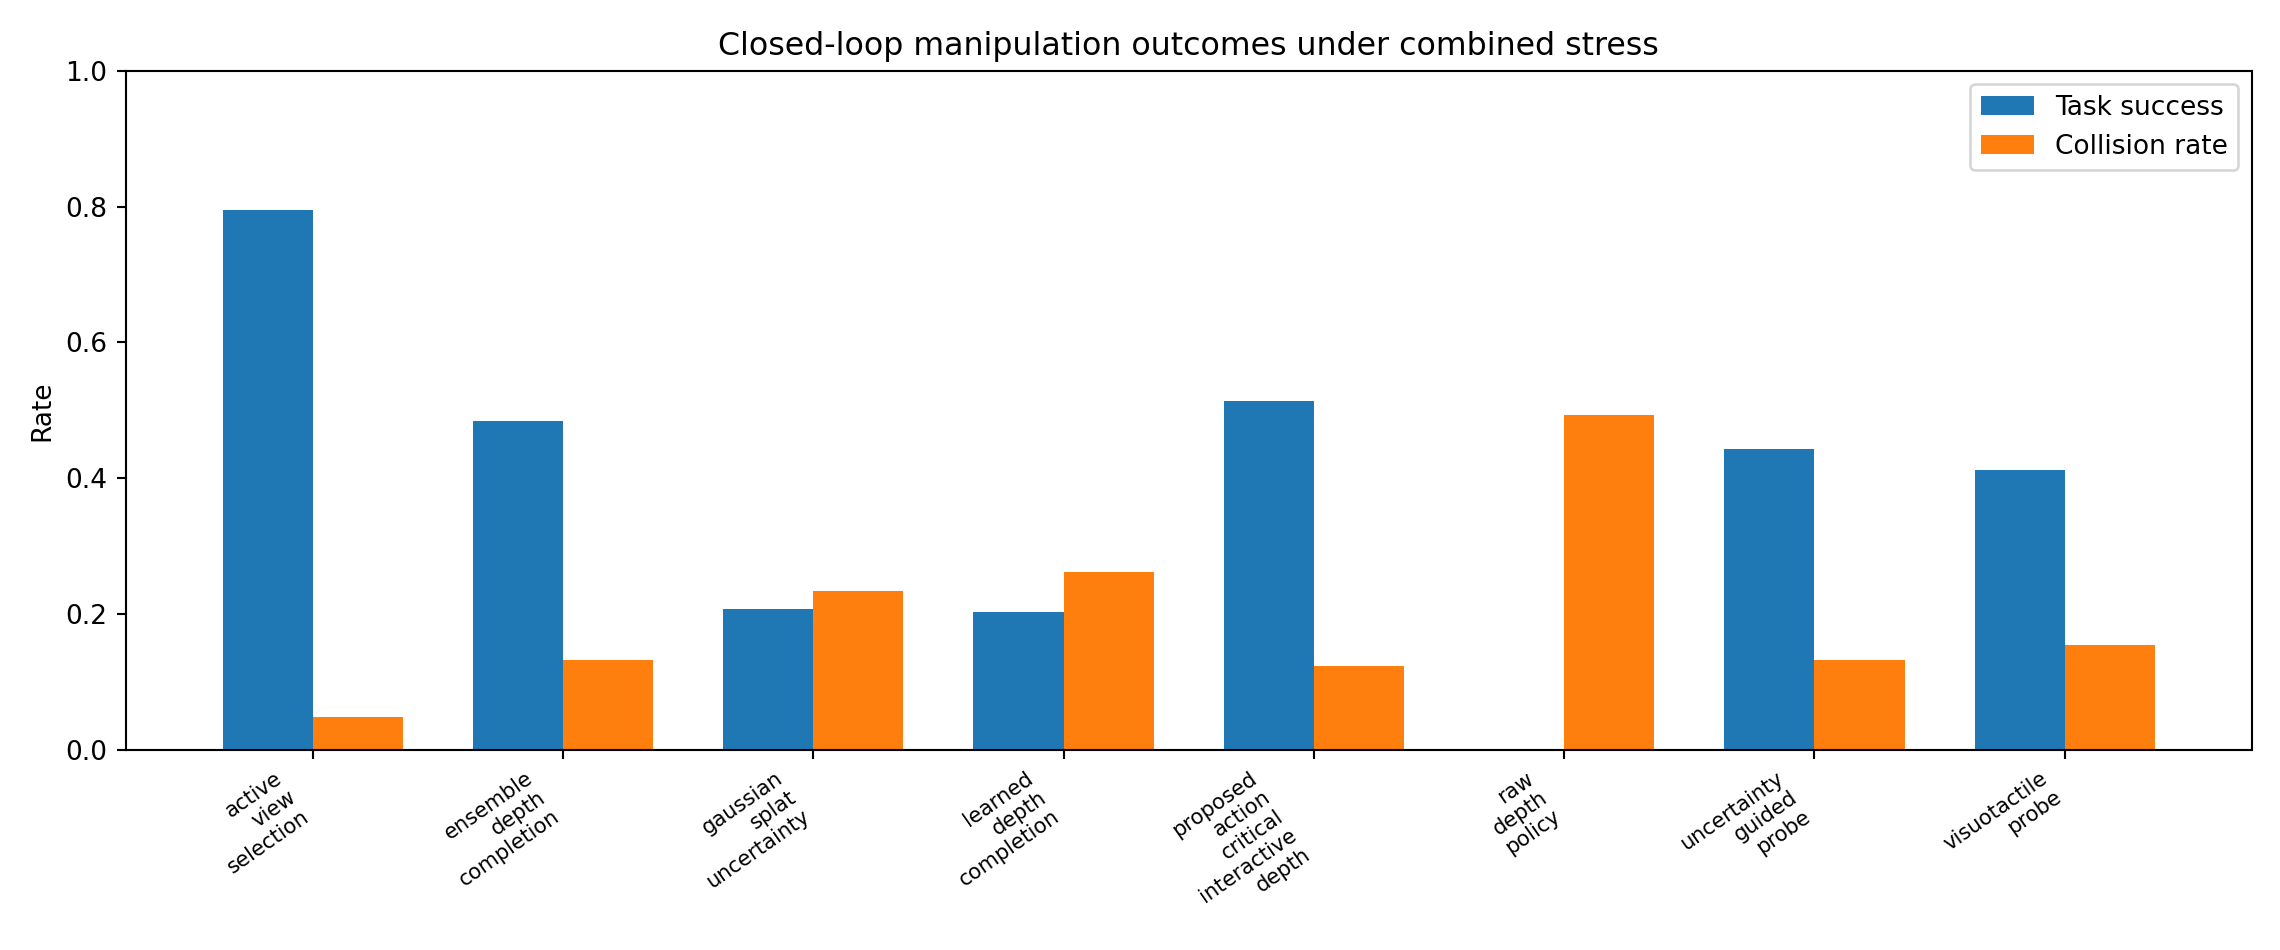
\includegraphics[width=\textwidth]{../figures/interactive_depth_task_outcomes.png}
\caption{Closed-loop outcomes under combined stress. The proposed method improves over several weak baselines but does not beat active view selection.}
\label{fig:outcomes}
\end{figure}

\begin{figure}[t]
\centering
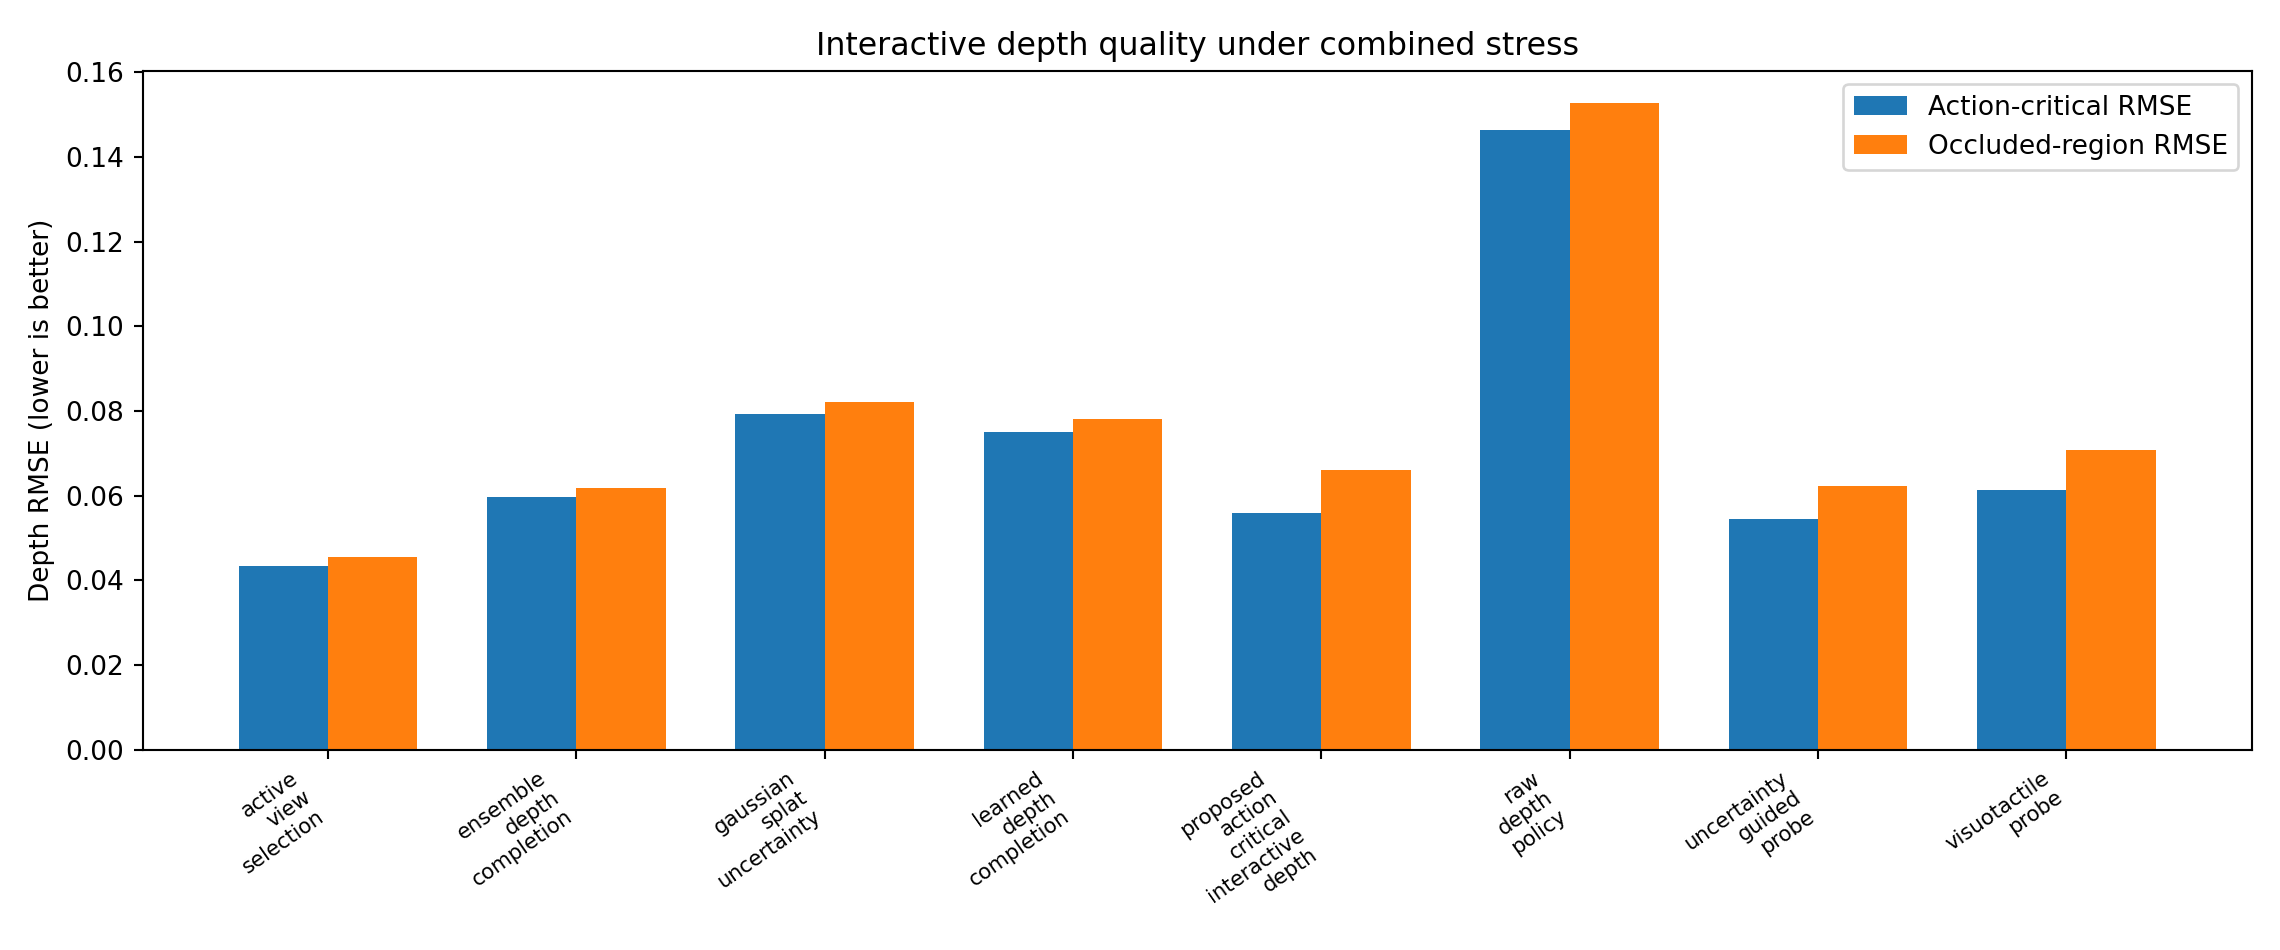
\includegraphics[width=\textwidth]{../figures/interactive_depth_quality.png}
\caption{Depth quality under combined stress. Active view selection also has lower action-critical RMSE than the proposed physical probing method.}
\label{fig:quality}
\end{figure}

\section{Paired Gate}

The strongest non-oracle baseline is active view selection. The proposed method loses on every gate metric:

\begin{table}[t]
\caption{Paired proposed-minus-active-view differences over 28 task/seed groups. Negative is good for success only; positive is worse for RMSE, collisions, regret, and damage.}
\label{tab:paired}
\centering
\resizebox{\textwidth}{!}{\begin{tabular}{llll}
\toprule
Metric & Comparator & Diff & CI95 \\
\midrule
task\_success & active\_view\_selection & -0.2807 & 0.0713 \\
action\_critical\_rmse & active\_view\_selection & 0.0126 & 0.0020 \\
collision\_rate & active\_view\_selection & 0.0754 & 0.0247 \\
planning\_regret\_to\_oracle & active\_view\_selection & 0.1741 & 0.0241 \\
probe\_damage & active\_view\_selection & 0.1528 & 0.0222 \\
\bottomrule
\end{tabular}
}
\end{table}

The decisive result is the success gap: proposed action-critical probing is lower by $0.28075 \pm 0.07128$. The RMSE gap is also unfavorable: proposed action-critical RMSE is higher by $0.01259 \pm 0.00203$. The safety metrics are not rescue signals; collisions, regret, and damage all increase relative to active view selection.

\section{Ablations}

The internal ablations partially support the intended mechanism: removing physical probing, action criticality, calibration, or cost control usually hurts the full method. However, internal ablation support cannot rescue the paper when an external non-contact baseline is stronger.

\begin{table}[t]
\caption{Ablations under combined stress. The full method is the best internal variant, but the external active-view baseline remains much stronger.}
\label{tab:ablations}
\centering
\resizebox{\textwidth}{!}{\begin{tabular}{lllll}
\toprule
Ablation & Success & AC-RMSE & Probe cost & Damage \\
\midrule
action\_only\_probe & 0.457 $\pm$ 0.101 & 0.058 & 0.066 & 0.149 \\
minus\_action\_criticality & 0.491 $\pm$ 0.099 & 0.059 & 0.066 & 0.161 \\
minus\_physical\_probe & 0.398 $\pm$ 0.104 & 0.067 & 0.000 & 0.000 \\
minus\_probe\_cost\_model & 0.445 $\pm$ 0.103 & 0.052 & 0.146 & 0.259 \\
minus\_uncertainty\_calibration & 0.481 $\pm$ 0.088 & 0.056 & 0.066 & 0.140 \\
proposed\_action\_critical\_interactive\_depth & 0.519 $\pm$ 0.097 & 0.056 & 0.066 & 0.146 \\
uncertainty\_only\_probe & 0.456 $\pm$ 0.104 & 0.059 & 0.123 & 0.218 \\
\bottomrule
\end{tabular}
}
\end{table}

\begin{figure}[t]
\centering
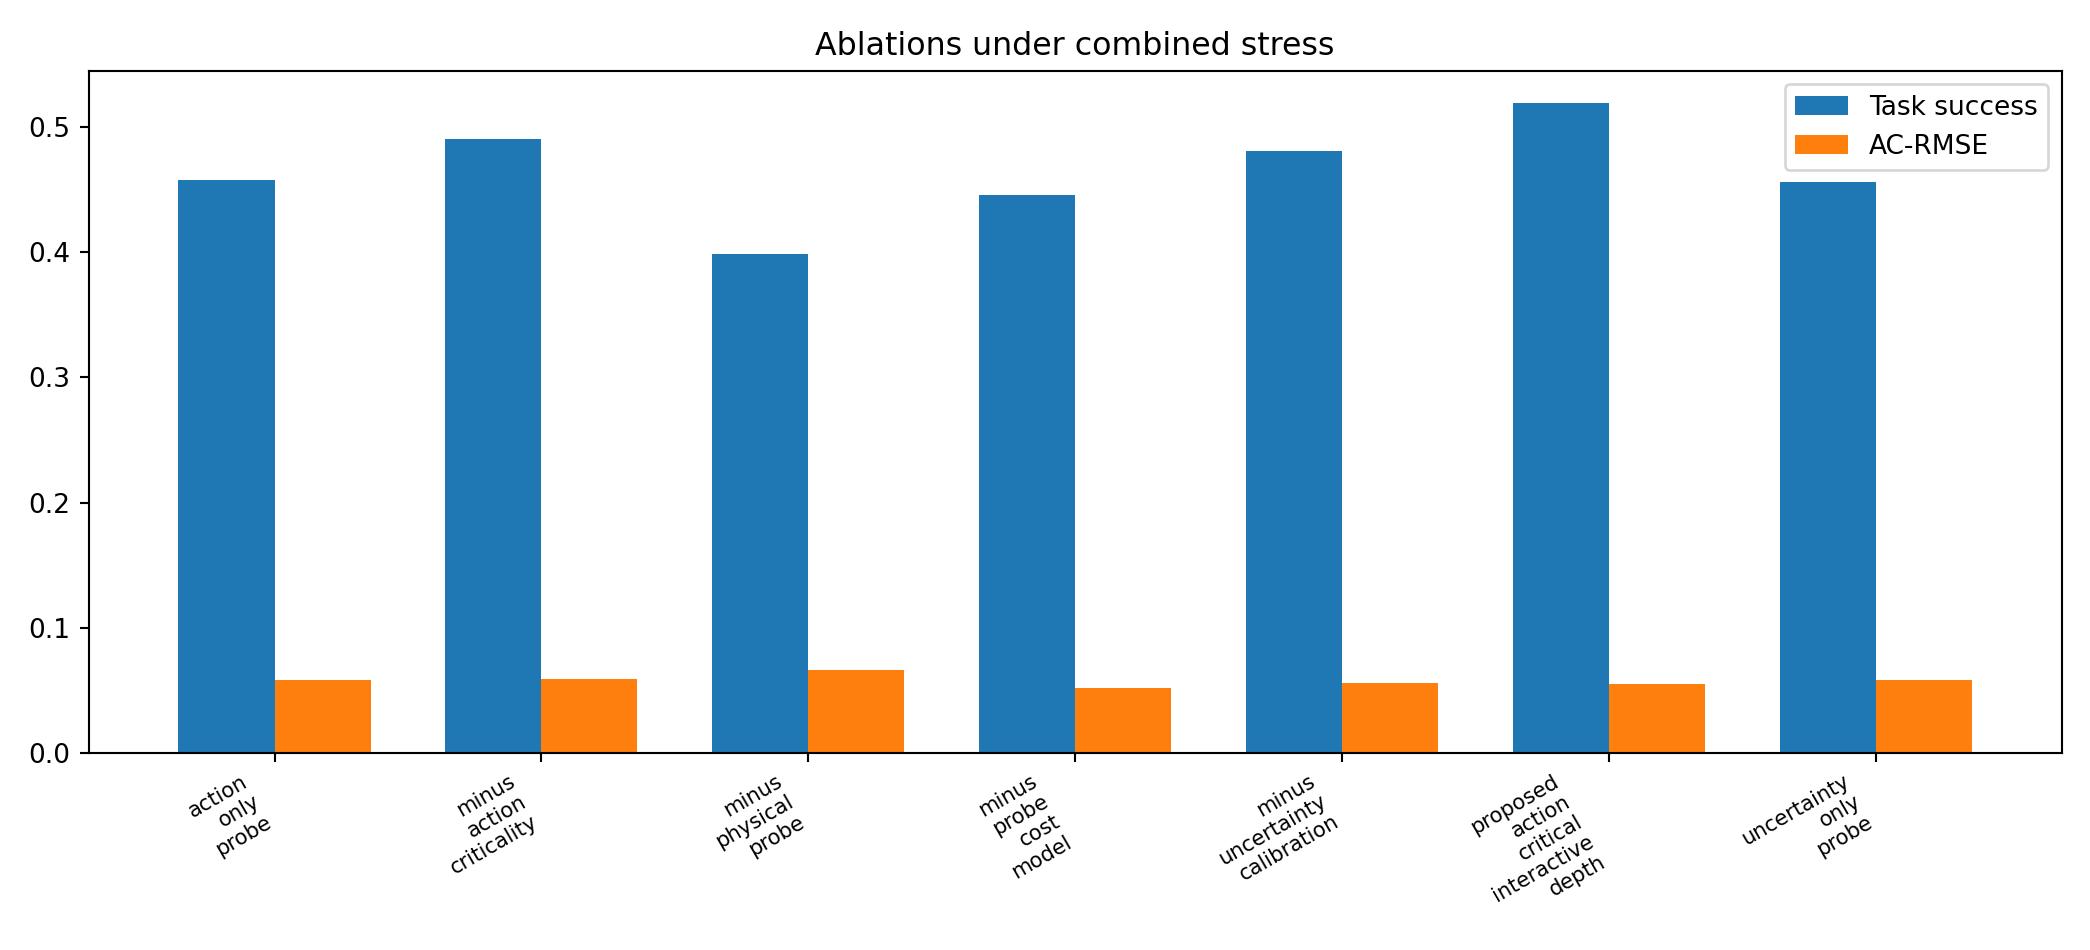
\includegraphics[width=\textwidth]{../figures/interactive_depth_ablation.png}
\caption{Ablation outcomes. The full method has a plausible internal mechanism, but this is not enough for submission readiness.}
\label{fig:ablations}
\end{figure}

\section{Stress Sweep and Cost-Regret Tradeoff}

The stress sweep reinforces the kill decision. At maximum stress, active view selection remains ahead at $0.780 \pm 0.084$ success, while proposed action-critical probing reaches $0.494 \pm 0.096$. The probe-based methods also accumulate contact damage as stress increases.

\begin{figure}[t]
\centering
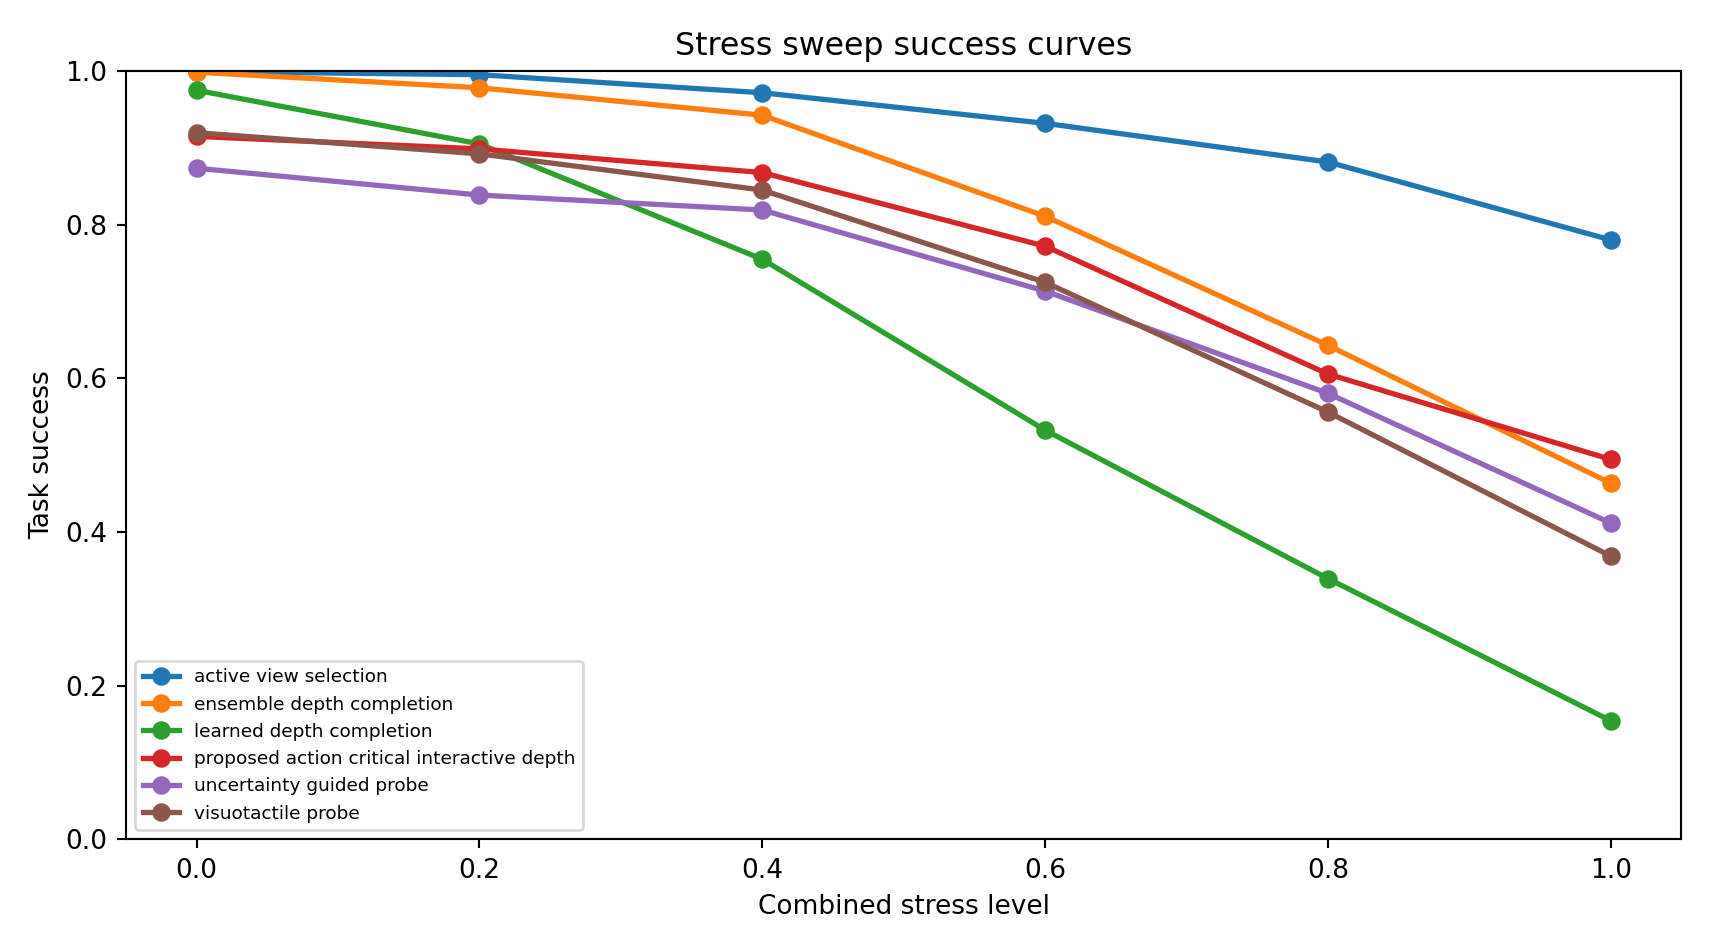
\includegraphics[width=\textwidth]{../figures/interactive_depth_stress_sweep.png}
\caption{Stress sweep. Active view selection degrades more gracefully than physical probing while avoiding damage.}
\label{fig:stress}
\end{figure}

\begin{figure}[t]
\centering
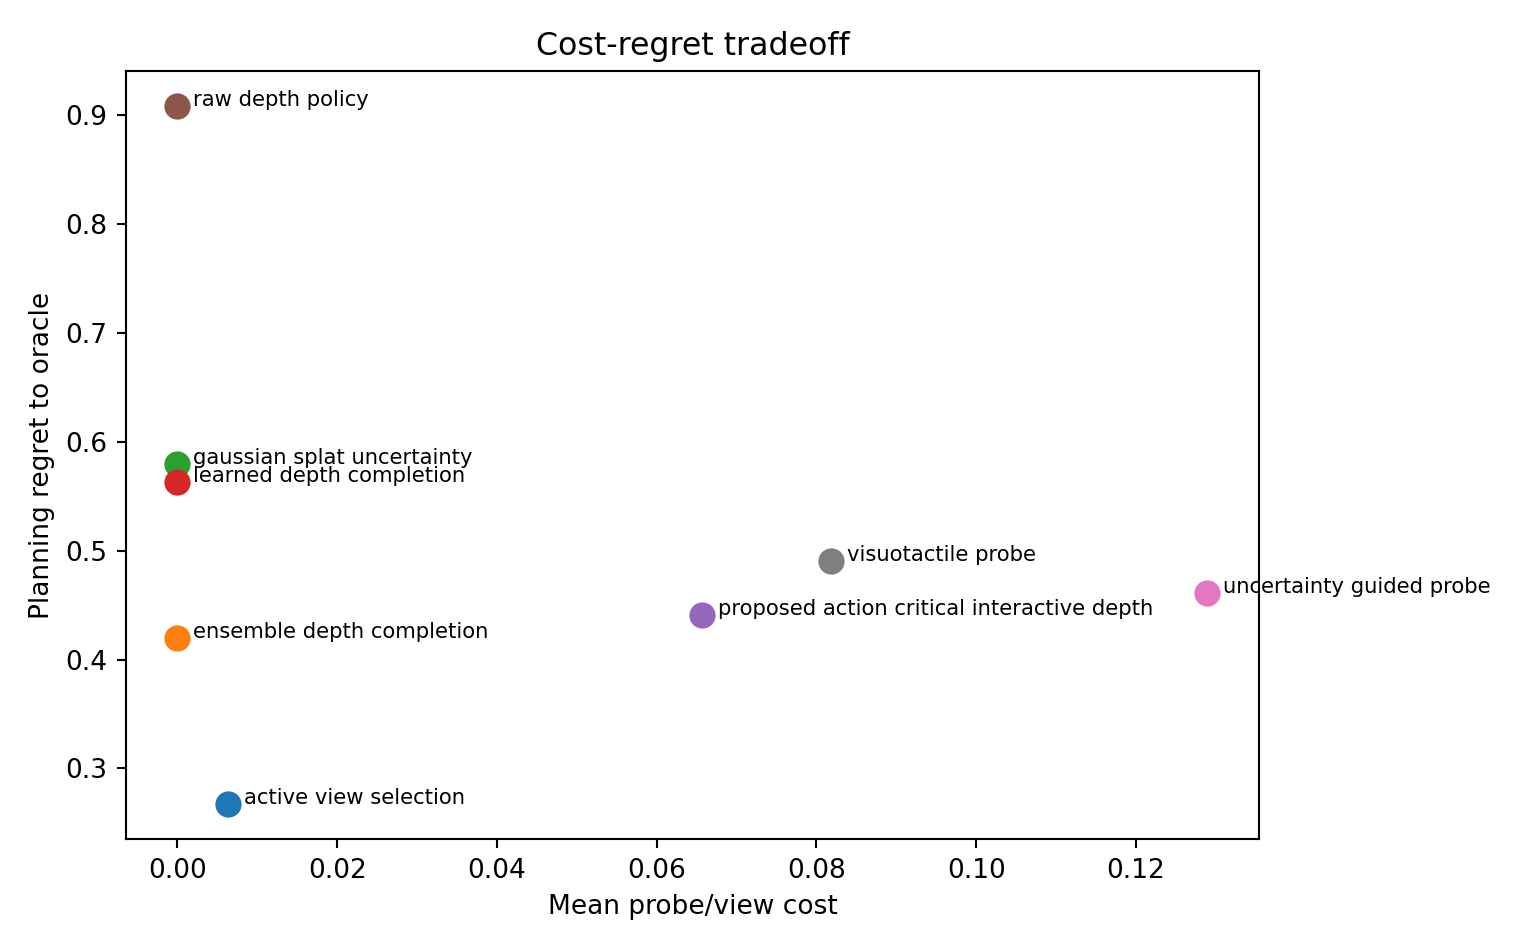
\includegraphics[width=0.86\textwidth]{../figures/interactive_depth_cost_regret.png}
\caption{Cost-regret tradeoff under combined stress. The proposed method pays more physical interaction cost and has higher regret than active view selection.}
\label{fig:costregret}
\end{figure}

\section{Failure Cases}

The proposed method fails for different reasons across tasks. In leaf-occluded fruit grasping, action-critical probing damages fragile targets: success is $0.230$, collision is $0.206$, and damage is $0.228$. In transparent container lifting, specular depth plus probe noise keeps success at $0.244$. In shelf insertion, tight clearance rewards conservative non-contact uncertainty handling. In occluded bin grasping, active view selection recovers enough geometry without touching objects.

\section{Limitations}

This audit is intentionally honest about its limits. The benchmark is deterministic and paper-specific, but it is still local simulation. It does not contain real-robot evidence, high-fidelity physics, trained checkpoints, external codebase integrations, hardware videos, or a manual full-paper related-work synthesis. Those missing items would already prevent an ICLR-main submission. More importantly, the available evidence is negative even before reaching that bar.

\section{Conclusion}

Interactive depth completion through action-critical physical probing is not ICLR-main ready. The proposed mechanism is plausible internally but loses to active view selection under the main stress gate. The correct terminal action is \textbf{KILL/ARCHIVE}. A revival would require a substantially new empirical project in which physical probing beats active view selection on task success, action-critical geometry, collision safety, planning regret, and damage/cost in real robot or high-fidelity simulator experiments.

\end{document}
